% Pattern Recognition Letters version. Rendered by paper/prl/render_prl.py from prl_template.tex:
% every number inside double braces is read from results/numbers.json, results/v2/numbers_v2.json
% or the result CSVs, and every table marked TABLE is built from the same files. Do not edit
% manuscript_prl.tex by hand; edit this template and re-render.
\documentclass[final,5p,times,twocolumn]{elsarticle}

\usepackage{amsmath,amssymb}
\usepackage{booktabs}
\usepackage{graphicx}
\usepackage{multirow}
\usepackage[hidelinks]{hyperref}
\usepackage{lineno}
\usepackage{textcomp}
\usepackage{microtype}

\journal{Pattern Recognition Letters}

\begin{document}

\begin{frontmatter}

\title{Seed-to-seed variation outweighs lightweight attention gains: a grouped, repeated cross-validation study on field durian disease images}

\author{Lin Ding Shan\corref{cor1}}
\ead{1002475487@ucsiuniversity.edu.my}
\cortext[cor1]{Corresponding author. ORCID: 0009-0009-6031-8479.}
\affiliation{organization={Institute of Computer Science and Digital Innovation, UCSI University},
             addressline={Jalan Menara Gading, UCSI Heights},
             city={Cheras},
             postcode={56000},
             state={Kuala Lumpur},
             country={Malaysia}}

\begin{abstract}
Attention modules are often reported to raise plant disease classification accuracy by a few points; we asked whether such gains can be measured on a small field dataset. An EfficientNet-B0 classifier of four durian disease classes was trained on 550 field images with and without three lightweight modules: a 1,281-parameter spatial gate (lesion-focus attention, LFA), squeeze-and-excitation (SE) and CBAM. Images were split by capture group; each configuration was trained on 20 grouped folds with two fixed seeds (160 runs) and compared in pairs with the corrected resampled $t$-test. Macro F1 was 75.1\% without attention and 74.9\%, 74.3\% and 74.7\% with LFA, SE and CBAM. No module met a decision rule fixed before the runs: the paired difference for LFA was $-$0.13 percentage points (95\% CI $-$4.56 to 4.31), also without the ungrouped video frames. Changing only the seed moved macro F1 by 5.34 points on average, and in 20\% of seed-matched single-run pairs LFA was at least 3 points ahead. A pre-registered 200-run follow-up varying insertion point and resolution found no gain. Single-run differences of a few points on data of this size are not evidence about the architecture.
\end{abstract}

\begin{keyword}
plant disease classification \sep attention mechanism \sep grouped cross-validation \sep random seed \sep corrected resampled $t$-test \sep durian
\end{keyword}

\end{frontmatter}

\section{Introduction}
\label{sec:intro}

Convolutional networks are now a standard approach to image-based plant disease diagnosis \cite{kamilaris2018deep}. Accuracy above 99\% has been reported, mostly on images taken under controlled conditions \cite{ferentinos2018deep,mohanty2016using}, and performance falls on photographs taken in the field, where background, lighting and symptom appearance vary \cite{barbedo2018impact,singh2020plantdoc}. Field datasets are also small, because each image has to be collected in an orchard and labelled by someone who can recognise the symptoms. Durian is a high-value fruit crop in Southeast Asia \cite{ogara2004botany}; its foliar, branch and trunk diseases include algal leaf spot, anthracnose and other leaf blights, \emph{Phomopsis} leaf spot, pink disease and \emph{Phytophthora} root and collar rot \cite{lim2003diseases}, and public image collections for the crop are recent and few \cite{nguyenthanh2025durian}.

A common way to improve such a classifier is to add an attention module, a small block that re-weights the feature maps of a pretrained network. Squeeze-and-excitation (SE) re-weights channels \cite{hu2018squeeze}, and the convolutional block attention module (CBAM) re-weights channels and spatial positions \cite{woo2018cbam}. In plant disease work, adding CBAM to EfficientNet-B0 and other pretrained networks has been reported to raise accuracy when training data are scarce \cite{alirezazadeh2023improving}. The reported gains are typically a few percentage points.

Gains of that size are hard to measure on a small field dataset, for three reasons. First, field photographs are not independent: a symptomatic leaf is usually photographed several times within a few seconds, and a random image-level split places near-identical views of one specimen on both sides of the split. This leakage inflates test scores \cite{kapoor2023leakage}, and the remedy is to split by the unit that generated the data \cite{beery2018recognition,roberts2017cross}. Second, training the same network twice with different random seeds gives different results, and the difference can be large relative to the effect being compared \cite{bouthillier2021accounting,picard2021torch}. Third, cross-validation folds share most of their training data, so a standard paired $t$-test over folds understates the variance and finds differences too easily \cite{dietterich1998approximate,nadeau2003inference}. On a few hundred images, each of these three sources is of the same order as the effect claimed for an attention module.

This letter asks whether lightweight attention improves the classification of field-photographed durian diseases when all three sources are controlled, and how large the uncontrolled sources would have been relative to the effect. An EfficientNet-B0 baseline was compared with three modules, a minimal spatial gate here called lesion-focus attention (LFA), SE and CBAM, under capture-group splits, 20 folds, two fixed seeds per fold, a corrected paired test and a decision rule written before the runs. A pre-registered follow-up tested whether the result depends on where the module is inserted or on the input resolution. The study also measured how far the score moves with the random seed alone, and tested the models without adaptation on an independent durian leaf dataset from Vietnam. The code, the fold assignment and every test prediction are released.

\section{Materials and methods}
\label{sec:methods}

\subsection{Images, classes and capture groups}
\label{sec:data}

The images were collected in commercial durian orchards in Peninsular Malaysia between July 2025 and June 2026, under ambient light and without background removal or standardised framing. Of the 560 released images, 526 carry the camera file-name prefix \texttt{IMG\_} and were taken by the author, mainly with one smartphone; 20 were sent by a grower through a messaging application, and 14 carry other file names. Labels were assigned by the author with guidance from growers and extension staff with field experience in these orchards. Identification rests on field symptoms, without isolation, culture or molecular confirmation, so the classes are symptom classes and not confirmed aetiologies. Ambiguous, low-quality and dual-infection images were excluded. Pink disease (\emph{Erythricium salmonicolor}), represented by ten images from three capture sessions, was excluded because a class of that size cannot be placed in every test fold or scored reliably. The remaining 550 images form four classes (Table~\ref{tab:classes}): algal leaf spot (\emph{Cephaleuros virescens}), leaf rot (a symptom cluster dominated by anthracnose, \emph{Colletotrichum} spp., together with other necrotic leaf blights that growers treat alike), \emph{Phomopsis} leaf spot, and root and collar rot (\emph{Phytophthora} spp.), which is photographed at the trunk base. Images were downscaled once to a longest edge of 512 pixels (Lanczos resampling, JPEG quality 92); for evaluation they were resized to 256 pixels on the short side and centre-cropped to $224 \times 224$.

\begin{table}[t]
\centering
\footnotesize
\caption{The four classes. A capture group is a set of photographs kept together in every split (Section~\ref{sec:data}). Five groups contain images of more than one class, so the class rows add up to more than the 60 groups in total. The last column is the share of each class held by its largest group; seven of the 14 \emph{Phomopsis} groups are single videos.}
\label{tab:classes}
\begin{tabular}{@{}llrrr@{}}
\toprule
Class & Organ & Images & Groups & Largest group (\%) \\
\midrule
Algal leaf spot & Leaf & 162 & 19 & 24.1 \\
Leaf rot & Leaf & 153 & 25 & 27.5 \\
\emph{Phomopsis} leaf spot & Leaf & 157 & 14 & 49.7 \\
Root and collar rot & Trunk base & 78 & 8 & 62.8 \\
\midrule
Total & & 550 & 60 & \\
\bottomrule
\end{tabular}
\end{table}

Photographs of one specimen taken seconds apart share the leaf, the background and the light; if they are split between training and test sets, the test score measures recognition of a specimen the model has already seen. Every image was therefore assigned to a capture group, and groups were never split. No specimen identifier was recorded at collection, so groups were reconstructed from file names. Frames extracted from one video formed one group. Camera files with the same name prefix whose sequence numbers were no more than three apart were joined into one burst, regardless of class and capture date. The rule is deliberately coarse: it joins consecutive photographs filed under different classes, and it joins photographs whose counter numbers coincide (32 camera file names, \texttt{IMG\_9885} to \texttt{IMG\_9972}, occur in two class folders for different photographs, and all 64 of these fall in one group). The 20 grower images were grouped by class, and the remaining files were singletons. These rules give 73 capture sessions within classes, 61 groups after joining across classes, and 60 groups after pink disease was removed. Groups are very unequal: the median group holds 4.5 images and the largest holds 128 (78 \emph{Phomopsis}, 42 leaf rot and 8 algal leaf spot images).

The video files also carry camera counter numbers, but they were not passed through the burst rule; this was an oversight. All 7 videos (63 frames) show \emph{Phomopsis} leaf spot and their counter numbers lie inside or next to the largest burst, so a video can fall in a different fold from still photographs taken just before or after it. Had the videos been joined by their counter numbers, the largest group would hold 202 images, including 152 of the 157 \emph{Phomopsis} images. The experiments were run with the groups as described; Section~\ref{sec:main} reports every comparison both on all test images and with the video frames excluded from scoring.

\subsection{Models}
\label{sec:models}

All models used EfficientNet-B0 \cite{tan2019efficientnet} with ImageNet weights \cite{deng2009imagenet}. The attention module was inserted after the last feature block, where the feature map $X \in \mathbb{R}^{C \times H \times W}$ has $C = 1280$ channels and $H = W = 7$ for a $224 \times 224$ input, and before global average pooling (Fig.~\ref{fig:arch}). The classifier was a dropout layer ($p = 0.3$) followed by a linear layer with four outputs. Four configurations were compared. \emph{None}: EfficientNet-B0 without an attention module (4.013\,M parameters). \emph{LFA}: a $1 \times 1$ convolution reduces the feature map to one channel, a logistic function turns it into a spatial weight map $A \in (0,1)^{H \times W}$, and the map multiplies every channel,
\begin{equation}
A_{hw} = \sigma\!\Big(\sum_{c=1}^{C} w_c X_{chw} + b\Big), \qquad X'_{chw} = A_{hw}\,X_{chw},
\label{eq:lfa}
\end{equation}
where $w \in \mathbb{R}^{C}$ and $b \in \mathbb{R}$ are learned and $\sigma$ is the logistic function; with $C = 1280$ the module adds $C + 1 =$ 1,281 parameters. LFA is the simplest form of spatial attention; it was designed to weight lesion regions, but nothing in its structure is specific to lesions. \emph{SE}: squeeze-and-excitation with reduction ratio 16 \cite{hu2018squeeze}, adding 204,800 parameters. \emph{CBAM}: channel attention with reduction ratio 16 followed by spatial attention with a $7 \times 7$ convolution \cite{woo2018cbam}, adding 204,898 parameters.

\begin{figure*}[t]
\centering
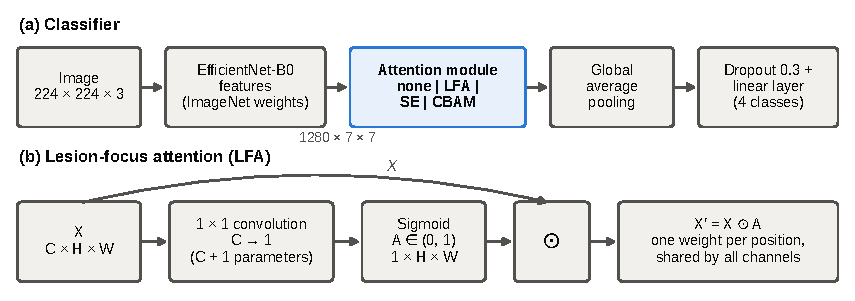
\includegraphics[width=\textwidth]{figs/fig1.pdf}
\caption{(a) Position of the attention module in the classifier. (b) The lesion-focus attention (LFA) module, Eq.~(\ref{eq:lfa}).}
\label{fig:arch}
\end{figure*}

\subsection{Training}
\label{sec:training}

Training followed a two-stage transfer-learning schedule. In stage~1 (15 epochs) the backbone weights were frozen and only the attention module and the classifier were trained, with Adam at a learning rate of $10^{-3}$; batch-normalisation statistics in the backbone continued to update because the network was in training mode. The checkpoint with the best inner-validation score was then loaded, all parameters were unfrozen, and stage~2 (15 epochs) continued at $10^{-5}$. The final model was the checkpoint with the highest inner-validation macro F1 over both stages. The batch size was 16. Class imbalance was handled with inverse-frequency class weights in the cross-entropy loss and a class-weighted random sampler. All four configurations used the same schedule and learning rates; no configuration was tuned separately. Training augmentation consisted of random resized cropping to 224 pixels (scale 0.7--1.0), horizontal and vertical flips, a random affine transformation (rotation up to $20^\circ$, translation up to 5\%, scale 0.95--1.05), colour jitter, Gaussian blur, ImageNet normalisation and random erasing; the full settings are listed in the supplementary material. Training used mixed precision on a Google Colab GPU runtime with PyTorch and torchvision \cite{paszke2019pytorch}. Each run was seeded: the seed fixed the Python, NumPy and PyTorch generators, the weighted sampler and the data-loader workers, and cuDNN was set to deterministic mode. Some GPU operations remain non-deterministic under these settings, so a rerun may differ slightly.

\subsection{Evaluation design and statistics}
\label{sec:eval}

The 550 images were split with stratified group $k$-fold cross-validation (scikit-learn \cite{pedregosa2011scikit}), with the capture group as the grouping variable and the class as the stratification variable. Four folds were used and the split was repeated five times with different shuffles, giving 20 test folds. Within the training part of each fold, about 10\% of the images were held out, again by whole groups, as an inner validation set for checkpoint selection, so that the test fold was used once, after training \cite{varma2006bias}. Because groups are unequal, fold sizes vary: the training sets held 247--459 images (mean 371.4), the inner validation sets 23--61 (mean 41.0) and the test folds 41--280 (mean 137.5). The largest root and collar rot group holds 49 of the 78 images of that class, and in 3 of the 20 folds no image of the class reached the test set. No group crossed a training, validation or test boundary in any fold. Each configuration was trained on every fold with two seeds (0 and 1), giving 160 runs; all configurations saw the same folds and seeds, so they can be compared in pairs.

The primary metric was macro F1 over the classes present in each test fold; accuracy was secondary. For each fold, the score of a configuration was the mean over its two seeds, and the effect of a module was the paired difference $d_j$ between the module and the plain network on fold $j$. The 20 differences were tested with the corrected resampled $t$-test of Nadeau and Bengio \cite{nadeau2003inference}, which inflates the variance of the mean by the factor $1/J + n_{\mathrm{test}}/n_{\mathrm{train}}$ to account for the overlap between training sets. Here $J = 20$ and $n_{\mathrm{test}}/n_{\mathrm{train}}$ was taken as the ratio of the mean test size to the mean training-plus-validation size, 137.5/412.5, so the factor is 0.383 against 0.05 for an ordinary paired test. The correction assumes a constant training-to-test ratio, which holds only approximately here; its use with repeated cross-validation follows Bouckaert and Frank \cite{bouckaert2004evaluating}. Uncorrected paired $t$-tests and Wilcoxon signed-rank tests are reported in the supplementary material.

Before the runs, a decision rule for LFA was written into the analysis notebook: LFA would count as an improvement only if its mean paired difference was at least 2 percentage points and the lower limit of the corrected 95\% confidence interval was above zero. The same rule is applied here to SE and CBAM. The rule was written for a macro F1 averaged over all four classes, which scores an absent class as zero; the present-class version reported here was computed afterwards from the saved predictions, and the two agree on every comparison (supplementary Table~S4). Two further quantities describe run-to-run variation: the \emph{seed difference}, the absolute difference in macro F1 between the two seeds of one configuration on one fold, and the \emph{single-run comparison}, which pairs each LFA run with the plain-network run of the same fold and seed and counts how often one is ahead by 3 points or more.

\subsection{Pre-registered follow-up: insertion point and input resolution}
\label{sec:followup}

The main experiment inserts the modules at the last feature map, where each of the $7 \times 7$ positions covers a large part of the leaf, and uses 224-pixel inputs, which may lose small lesions. After the main results were known, a follow-up tested both factors for LFA on the same 20 folds, seeds and schedule, with five configurations: the plain network at 224 pixels, rerun as the reference; LFA after feature block~5 (112 channels, stride 16, a $14 \times 14$ map; 113 parameters) and after block~3 (40 channels, stride 8, $28 \times 28$; 41 parameters) at 224 pixels; and the plain network and LFA after block~5 at 320 pixels. This gave 200 runs. The analysis was written down before the runs and is released with the results: each of the four configurations was compared with the 224-pixel plain network by the corrected test, the four $p$-values were Holm-adjusted, and a configuration would count as an improvement only if its mean paired difference was at least 2 points and the adjusted $p$ was below 0.05.

\subsection{External test and computational cost}
\label{sec:external}

To see whether a module helps when the image source changes, the models were evaluated without adaptation on the durian leaf dataset of Nguyen Thanh et al.\ \cite{nguyenthanh2025durian}, collected in Vietnam, whose images were cropped to a square and resized to $400 \times 400$ pixels by the dataset authors. Three of its foliar classes correspond to classes here: algal leaf spot (462 images), leaf rot (Leaf\_Blight, 440, and Leaf\_Colletotrichum, 400) and \emph{Phomopsis} leaf spot (411), counted as published. Its \emph{Rhizoctonia} class shows foliar symptoms while the corresponding class here is photographed at the trunk base, and its healthy class has no counterpart, so neither was used. After byte-identical duplicates were removed, 1,701 images remained; they were re-encoded as JPEG and passed through the same evaluation transform as the Malaysian images. A classifier guessing uniformly among the three shared classes would reach a macro F1 of about 32.5\%, and one guessing among four classes about 27.9\%. For this test each configuration was trained with five seeds on 488 of the 550 Malaysian images, with the remaining 62, taken as whole groups, used for checkpoint selection. Parameters were counted from the models, multiply--accumulate operations with the PyTorch FLOP counter for one $224 \times 224$ image, and CPU latency at batch size 1 on the Colab runtime (30 warm-up passes, then five interleaved rounds of 40 passes per model; median reported).

\section{Results}
\label{sec:results}

\subsection{No module measurably improved on the plain network}
\label{sec:main}

All four configurations reached a mean macro F1 of about 75\% on all test images and about 66\% when the video frames were excluded from scoring (Table~\ref{tab:main}). The paired differences from the plain network were close to zero for all three modules under both scorings, and every confidence interval included zero (Fig.~\ref{fig:main}a). The mean difference for LFA was $-$0.13 percentage points (95\% CI $-$4.56 to 4.31) on all images and $-$0.13 ($-$4.55 to 4.28) without the frames; LFA scored higher than the plain network on 11 of 20 folds. SE and CBAM had mean differences of $-$0.77 and $-$0.38 points on all images, with wider intervals. None of the modules met the decision rule, and neither the uncorrected $t$-test nor the Wilcoxon test detected a difference (all $p \geq 0.27$). Accuracy gave the same result, with paired differences of $-$0.49 (LFA), $-$1.20 (SE) and $-$0.17 points (CBAM). A stricter check that scored only test images whose group would not have been split had the videos been linked gave a difference of $-$0.83 points for LFA (95\% CI $-$6.09 to 4.44), although almost no \emph{Phomopsis} images remain in that subset. A preliminary experiment with an earlier version of the code, eight runs per configuration on one fixed split of all five classes, had shown the same pattern (supplementary Table~S3).

With confidence-interval half-widths of 4.4--6.8 points, the decision rule could have been met only by gains of about 4.4 points or more for LFA, and larger gains for SE and CBAM. The modules added little computation: LFA added 1,281 parameters and about 0.0001 GMACs; SE and CBAM each added about 0.2 million parameters, 5.1\% of the network. Relative to the plain network, single-thread CPU latency changed by $-$0.11\,ms (LFA), $-$0.08\,ms (SE) and +0.91\,ms (CBAM) on a median of 34.3\,ms (supplementary Table~S8).

\begin{table*}[t]
\centering
\footnotesize
\caption{Macro F1 over 160 runs (40 per configuration; mean $\pm$ SD) and paired difference from the plain network over 20 folds, scored on all test images and with the 63 video frames excluded. CI and $p$ from the corrected resampled $t$-test; ``Folds higher'' counts the folds on which the module beat the plain network (all images). Accuracy is in supplementary Table~S2.}
\label{tab:main}
\begin{tabular}{@{}lrlrrlrr@{}}
\toprule
 & \multicolumn{3}{c}{All test images} & \multicolumn{3}{c}{Video frames excluded} & \\
\cmidrule(lr){2-4}\cmidrule(lr){5-7}
Configuration & Macro F1 (\%) & Difference (pp) [95\% CI] & $p$ & Macro F1 (\%) & Difference (pp) [95\% CI] & $p$ & Folds higher \\
\midrule
None & 75.06 $\pm$ 10.86 & -- & -- & 66.60 $\pm$ 12.04 & -- & -- & -- \\
LFA & 74.93 $\pm$ 10.95 & $-$0.13 [$-$4.56, 4.31] & 0.953 & 66.46 $\pm$ 12.15 & $-$0.13 [$-$4.55, 4.28] & 0.950 & 11/20 \\
SE & 74.29 $\pm$ 11.80 & $-$0.77 [$-$7.62, 6.08] & 0.816 & 65.34 $\pm$ 12.74 & $-$1.26 [$-$10.28, 7.76] & 0.773 & 10/20 \\
CBAM & 74.68 $\pm$ 10.78 & $-$0.38 [$-$5.48, 4.73] & 0.879 & 66.37 $\pm$ 13.06 & $-$0.23 [$-$5.83, 5.37] & 0.933 & 8/20 \\
\bottomrule
\end{tabular}
\end{table*}

\begin{figure*}[t]
\centering
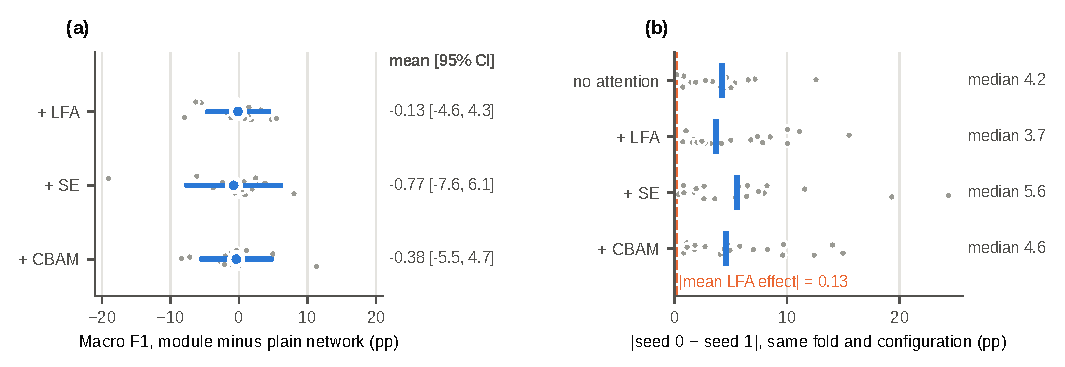
\includegraphics[width=\textwidth]{figs/fig2.pdf}
\caption{(a) Paired difference in macro F1 between each attention module and the plain network, all test images. Each grey point is one of the 20 folds (mean of two seeds); blue, mean and 95\% confidence interval of the corrected resampled $t$-test. (b) Absolute difference in macro F1 between the two seeds of the same configuration on the same fold (20 folds per configuration); blue bars, medians; dashed line, absolute mean effect of LFA from panel (a).}
\label{fig:main}
\end{figure*}

\subsection{Run-to-run variation}
\label{sec:variation}

Changing only the random seed, with the configuration and the fold held fixed, changed macro F1 by 5.34 points on average (median 4.41, maximum 24.36; Fig.~\ref{fig:main}b). The median seed difference was 4.21 points for the plain network, 3.69 for LFA, 5.56 for SE and 4.57 for CBAM. Without the video frames the seed difference averaged 5.67 points, so this variation does not come from the frames. The typical seed difference is larger than the 2-point threshold of the decision rule and comparable to the half-width of the confidence intervals.

In the single-run comparison, LFA was at least 3 points ahead of the plain network in 8 of 40 seed-matched pairs (20\%) and at least 3 points behind in another 8 (20\%); the difference within a pair ranged from $-$13.35 to +16.77 points. For SE the corresponding shares were 30\% ahead and 25\% behind, and for CBAM 17.5\% each. The 40 pairs are not independent, since two come from each fold, so these shares are rough. The absolute score also depended strongly on the test fold: fold means, averaged over configurations and seeds, ranged from 50.0\% to 92.8\% (SD 10.15), whereas the four configuration means differed by less than one point (SD 0.34). The paired design removes this fold effect from the comparison of configurations, but the spread shows how much a score from one grouped split depends on which groups happen to be tested.

\subsection{Insertion point and input resolution}
\label{sec:followup_res}

Neither factor produced a gain that met the pre-registered rule (Table~\ref{tab:followup}). Moving LFA to the $14 \times 14$ map lowered mean macro F1 by 1.51 points (95\% CI $-$6.30 to 3.28) and to the $28 \times 28$ map by 2.75 points ($-$8.52 to 3.01); LFA was higher than the plain network on only 7 and 6 of the 20 folds. Raising the input to 320 pixels gave the largest mean change, +1.77 points, but the interval ($-$4.33 to 7.88) included zero. Adding LFA at 320 pixels did not help (+0.23 against the 224-pixel reference; $-$1.54, 95\% CI $-$8.52 to 5.43, against the 320-pixel plain network). After Holm adjustment every $p$ was 1.0. The rerun plain network scored 75.30\% against 75.06\% in the main experiment, and the mean seed difference was 5.61 points, in line with Section~\ref{sec:variation}.

\begin{table}[t]
\centering
\footnotesize
\setlength{\tabcolsep}{3.5pt}
\caption{Pre-registered follow-up (200 runs; 40 per configuration): LFA at earlier insertion points and at a higher input resolution. Mean $\pm$ SD of macro F1 and paired difference from the 224-pixel plain network over 20 folds, corrected test, Holm adjustment over the four comparisons.}
\label{tab:followup}
\resizebox{\columnwidth}{!}{%
\begin{tabular}{@{}lrlrr@{}}
\toprule
Configuration & Macro F1 (\%) & Difference (pp) [95\% CI] & $p_{\mathrm{Holm}}$ & Folds higher \\
\midrule
None, 224 px & 75.30 $\pm$ 11.02 & -- & -- & -- \\
LFA after block 5 ($14{\times}14$), 224 px & 73.79 $\pm$ 11.31 & $-$1.51 [$-$6.30, 3.28] & 1.000 & 7/20 \\
LFA after block 3 ($28{\times}28$), 224 px & 72.55 $\pm$ 11.42 & $-$2.75 [$-$8.52, 3.01] & 1.000 & 6/20 \\
None, 320 px & 77.08 $\pm$ 11.26 & +1.77 [$-$4.33, 7.88] & 1.000 & 15/20 \\
LFA after block 5 ($20{\times}20$), 320 px & 75.54 $\pm$ 12.69 & +0.23 [$-$7.39, 7.86] & 1.000 & 8/20 \\
\bottomrule
\end{tabular}}
\end{table}

\subsection{Per-class behaviour and external test}
\label{sec:perclass}

Root and collar rot reached the highest F1 (93.6\% without attention, recall 99.3\%; Table~\ref{tab:perclass}). It is the only class photographed at the trunk base and 63\% of its images come from one capture group, so its score probably reflects the organ and background as much as the symptoms. The three foliar classes were harder. Algal leaf spot had the lowest F1 (65.3\%), mainly through low recall: in the pooled predictions 23.8\% of algal leaf spot images were classified as leaf rot, as were 23.2\% of \emph{Phomopsis} images. The \emph{Phomopsis} scores are inflated by the video frames: the plain network recognised 95.7\% of \emph{Phomopsis} video frames but only 41.5\% of \emph{Phomopsis} still photographs. LFA changed per-class F1 by at most 1.8 points and recall by at most 4.0 points, within the run-to-run spread (supplementary Table~S1 and Fig.~S1).

\begin{table}[t]
\centering
\footnotesize
\setlength{\tabcolsep}{4pt}
\caption{Per-class precision, recall and F1 (\%, mean $\pm$ SD over runs) for the plain network and LFA, all test images. Root and collar rot was present in the test set in 34 of 40 runs per configuration, the other classes in all 40. \emph{Phomopsis} values include the video frames (Section~\ref{sec:perclass}). SE and CBAM are in supplementary Table~S1.}
\label{tab:perclass}
\begin{tabular}{@{}llrrr@{}}
\toprule
Class & Config. & Precision & Recall & F1 \\
\midrule
Algal leaf spot & None & 72.9 $\pm$ 25.5 & 63.7 $\pm$ 18.4 & 65.3 $\pm$ 19.3 \\
 & LFA & 73.8 $\pm$ 25.9 & 61.1 $\pm$ 21.2 & 63.6 $\pm$ 21.0 \\
Leaf rot & None & 66.6 $\pm$ 15.4 & 78.9 $\pm$ 16.0 & 70.7 $\pm$ 12.3 \\
 & LFA & 66.9 $\pm$ 16.2 & 82.9 $\pm$ 15.1 & 71.8 $\pm$ 11.1 \\
\emph{Phomopsis} leaf spot & None & 77.2 $\pm$ 20.5 & 78.6 $\pm$ 19.0 & 74.2 $\pm$ 13.4 \\
 & LFA & 77.7 $\pm$ 20.2 & 76.7 $\pm$ 19.4 & 73.5 $\pm$ 13.9 \\
Root and collar rot & None & 91.0 $\pm$ 18.3 & 99.3 $\pm$ 2.1 & 93.6 $\pm$ 14.2 \\
 & LFA & 92.3 $\pm$ 16.2 & 99.0 $\pm$ 2.2 & 94.6 $\pm$ 11.6 \\
\bottomrule
\end{tabular}
\end{table}

On the Vietnamese images, all four configurations reached a macro F1 of 39--41\% over the three shared classes (Table~\ref{tab:external}), against 27.9--32.5\% for random guessing and about 66--75\% in the Malaysian cross-validation. Fewer than 1\% of the Vietnamese images were classified as root and collar rot, so masking that class changed the means by at most 0.2 points. LFA and SE scored slightly higher than the plain network (+1.15 and +1.10 points) and CBAM slightly lower ($-$0.45), but none of these differences was reliable across five seeds (paired $t$-test $p = 0.32$, 0.36 and 0.73). The models transfer poorly to these images, and the test is too insensitive to separate the modules.

\begin{table}[t]
\centering
\footnotesize
\caption{Zero-shot macro F1 on 1,701 images of the Vietnamese dataset (three shared classes, four-class output; mean $\pm$ SD over five seeds) and paired difference from the plain network. Random guessing would score about 27.9\%.}
\label{tab:external}
\begin{tabular}{@{}lrrrr@{}}
\toprule
Configuration & Macro F1 (\%) & Diff.\ (pp) & $p$, paired $t$ & Seeds higher \\
\midrule
None & 39.82 $\pm$ 2.52 & -- & -- & -- \\
LFA & 40.97 $\pm$ 3.28 & +1.15 & 0.317 & 4/5 \\
SE & 40.92 $\pm$ 1.00 & +1.10 & 0.359 & 3/5 \\
CBAM & 39.36 $\pm$ 0.91 & $-$0.45 & 0.731 & 3/5 \\
\bottomrule
\end{tabular}
\end{table}

\section{Discussion}
\label{sec:discussion}

None of the three attention modules measurably improved the plain EfficientNet-B0 on the Malaysian images, and the confidence intervals exclude gains larger than about 4.3 points for LFA, 6.1 for SE and 4.7 for CBAM. The study cannot say why. The first explanation considered was the insertion point: at $7 \times 7$ resolution each position covers a large part of the leaf, and global average pooling already combines all positions. The follow-up does not support it: LFA on $14 \times 14$ and $28 \times 28$ maps scored lower, not higher. A higher input resolution raised the mean by about 1.8 points but not reliably, and LFA did not add to it. A second explanation is the amount of data: with about 370 training images per fold and no separate tuning, the extra parameters of SE and CBAM may be hard to train well, and a single-channel gate trained from random initialisation on a few hundred images may simply learn little. Other backbones and module-specific learning rates were not tested. Alirezazadeh et al.\ \cite{alirezazadeh2023improving} found that CBAM improved pretrained networks, including EfficientNet-B0, on a leaf dataset of about 3,000 images, with data and an evaluation design different from those used here; on the present field images a gain of a few points would not have been detectable without controlling the split, the seed and the test, and no gain appeared when they were controlled.

The result that carries over to other small field datasets is the size of the uncontrolled variation. The seed alone moved macro F1 by about 5 points on average, more than the 2-point threshold of the decision rule and about as much as the half-width of the confidence intervals. If a module had no average effect, a study that trained each configuration once on one grouped split could still have seen a difference of 3 points or more in its favour about one time in five. A gain of that size from a single comparison on a dataset of this size is therefore weak evidence about the architecture. For datasets like this one it helps to split images by the unit that generated them, to train each configuration with several seeds on several folds, to compare configurations in pairs on the same folds and seeds, and to use a test that allows for overlapping training sets. Here the corrected and uncorrected tests agreed, so the conclusion does not depend on that choice; because the corrected intervals were 9--14 points wide, much larger designs would be needed to detect gains of 1--2 points. Since the four configurations performed alike, the plain network is the simplest choice; among the modules LFA is the cheapest, with 1,281 parameters and no measurable latency.

The study has limits. It used one backbone and one training schedule for all configurations; the insertion point and input resolution were varied only for LFA, after the main results were known, with the analysis fixed in advance. The data come from one collection of 550 images labelled by one person on the basis of field symptoms, without a second rater. Capture groups were reconstructed from file names and are deliberately coarse, and the video frames were not linked to the photographs taken with them. The comparison between configurations was insensitive to this, but the absolute scores on all images are optimistic, and the scoring without frames is the better estimate; linked properly, almost all \emph{Phomopsis} images would form one group, so the dataset contains few independent capture events for that class, and no grouped split of these data can test how well it generalises. Groups may also miss other links, such as photographs of one tree taken on two visits. Three of the 20 test folds contained no root and collar rot image, and that class is probably recognised partly by organ and background. The primary metric was changed from the four-class to the present-class macro F1 after the runs, and the decision rule was written for LFA only; the conclusions are the same under both metrics. Orchard identity was not recorded per image, so generalisation to unseen orchards could not be tested. The Vietnamese images differ in preprocessing as well as origin, and all models scored not far above chance on them. Finally, two seeds per fold were used; more seeds would narrow the estimate of run-to-run variation but would not remove the fold-to-fold variation, which comes from the small number of independent capture groups.

\section{Conclusion}
\label{sec:conclusion}

On 550 field images of four durian disease classes, evaluated with capture-group splits, 20 folds, fixed seeds and paired corrected tests, there was no evidence that LFA, SE or CBAM improves an EfficientNet-B0 classifier; gains larger than about 4--6 points are excluded, smaller ones are not. Moving LFA to earlier layers or raising the input resolution did not change this. Changing only the random seed moved macro F1 by about 5 points on average, so differences of a few points between single runs on data of this size say little about the architectures being compared. All models transferred poorly to an independent Vietnamese dataset, which therefore could not separate them.

\section*{CRediT authorship contribution statement}
\textbf{Lin Ding Shan:} Conceptualization, Methodology, Software, Validation, Formal analysis, Investigation, Data curation, Writing -- original draft, Writing -- review \& editing, Visualization.

\section*{Declaration of competing interest}
The author is developing a handheld decision-support device for durian disease and pest scouting and therefore has a potential financial interest in the field this study evaluates. The author declares no other competing interests.

\section*{Funding}
This research did not receive any specific grant from funding agencies in the public, commercial, or not-for-profit sectors.

\section*{Data availability}
The 560 images and their capture-session identifiers are available on Zenodo (\url{https://doi.org/10.5281/zenodo.22177133}). The code, the fold assignment, all per-image test predictions, the pre-registered analysis of the follow-up and the scripts that regenerate every number, table and figure in this letter are available at \url{https://github.com/xiaolin200206/durian-attention-cv}. The Vietnamese dataset is available from its authors \cite{nguyenthanh2025durian}.

\section*{Ethics statement}
The study involved no human participants or animals. Access to the orchards was granted by their owners.

\section*{Acknowledgements}
The author thanks the orchard owners who allowed access to their orchards, and the growers and extension staff who helped define the symptom classes.

\section*{Declaration of generative AI and AI-assisted technologies in the writing process}
During the preparation of this work the author used Claude (Anthropic) to help write and check the experiment and analysis code and to edit the text of the manuscript. The author designed the study, collected and labelled the images, ran all training, checked every script and result, and after using this tool reviewed and edited the content as needed and takes full responsibility for the content of the publication.

\bibliographystyle{elsarticle-num}
\bibliography{refs}

\end{document}
